\section{Two-Stage Recommendation Engine and Algorithmic Formulation}

\subsection{Two-Stage Architectural Rationale}
Evaluating the full Cartesian product space $|U| \times |I| \approx 1.37 \times 10^6 \times 105,542 \approx 1.44 \times 10^{11}$ candidate pairs under complex ensemble tree models in real time is computationally intractable within sub-$100\,\text{ms}$ latency budgets. To achieve industrial scalability, HUB formalizes a \textbf{Two-Stage Recommendation Pipeline} following industry best practices \cite{covington2016deep}:
\begin{enumerate}
    \item \textbf{Stage 1 (Candidate Retrieval):} Reduces the universal catalogue ($|I| \approx 105,100$) to a personalized candidate subset of $C=100$ high-potential candidates per user using multi-heuristic retrieval channels (Recall@100 $= 79.43\%$).
    \item \textbf{Stage 2 (Pointwise Ranking \& In-Session Re-ranking):} Scores each candidate pair through a 200-tree \textbf{Random Forest Ranker} to estimate posterior purchase probabilities $\hat{p}(u, i)$, subsequently adjusted in real time by an exponential half-life session decay model.
\end{enumerate}

\subsection{Algorithmic Formalization of Stage 1 Retrieval}
The candidate retrieval and training dataset construction workflow is rigorously defined in Algorithm \ref{algo:stage1_retrieval}.

\begin{algorithm}[H]
\SetAlgoLined
\DontPrintSemicolon
\KwIn{Customer $u$, Transaction History $\mathcal{D} = \{(u', i', t') \mid t' < T_{\text{cutoff}}\}$, Item Catalog $I$, Age Cohorts $\mathcal{A}$, Negative Ratio $\lambda = 5$}
\KwOut{Training tuple set $\mathcal{T}_u$ of labeled candidate pairs $(u, i, y)$ where $y \in \{0, 1\}$}
$C_u \leftarrow \emptyset$\;
$C_{\text{repurchase}} \leftarrow \{i \in I \mid \exists (u, i, t) \in \mathcal{D} \text{ with } t \ge T_{\text{cutoff}} - 28\text{ days}\}$\;
$C_{\text{bestseller}} \leftarrow \operatorname{TopK}\big(\{i \in I \mid \operatorname{SalesCount}(i, [T_{\text{cutoff}}-7, T_{\text{cutoff}}])\}, K=12\big)$\;
$C_{\text{age}} \leftarrow \operatorname{TopK}\big(\{i \in I \mid \operatorname{SalesCountByAge}(i, \operatorname{AgeGroup}(u))\}, K=8\big)$\;
$C_{\text{copurchase}} \leftarrow \{j \in I \mid \exists i \in C_{\text{repurchase}} \text{ with } \operatorname{CoPurchased}(i, j) \ge 5\}$\;
$C_u \leftarrow (C_{\text{repurchase}} \cup C_{\text{bestseller}} \cup C_{\text{age}} \cup C_{\text{copurchase}})$ truncated to $C=100$\;
$Y_{\text{true}} \leftarrow \{i \in I \mid \exists (u, i, t) \in \mathcal{D} \text{ with } t \in [T_{\text{cutoff}}, T_{\text{cutoff}} + 7\text{ days}]\}$\;
$\text{Positives} \leftarrow \{(u, i, 1) \mid i \in (C_u \cap Y_{\text{true}})\}\;
\text{NegCandidates} \leftarrow C_u \setminus Y_{\text{true}}\;
\text{Negatives} \leftarrow \operatorname{SampleWithoutReplacement}\big(\text{NegCandidates}, \min(|\text{NegCandidates}|, \lambda \cdot |\text{Positives}|)\big)\;
\Return $\text{Positives} \cup \{(u, j, 0) \mid j \in \text{Negatives}\}$\;
\caption{Stage 1 Multi-Channel Candidate Retrieval and Controlled Negative Sampling}
\label{algo:stage1_retrieval}
\end{algorithm}

\subsection{Stage 2 Pointwise Random Forest Formulation}
The scoring stage formulates recommendation as a supervised binary classification problem. An ensemble of $B=200$ decision trees $T_b(\mathbf{x}_{u,i})$ is constructed via bootstrap aggregation (bagging) with random feature sub-selection:
\begin{equation}
    \hat{p}(u, i) = \frac{1}{B} \sum_{b=1}^{B} T_b\big(\mathbf{x}_{u,i}; \Theta_b\big), \quad \Theta_b = \{S_b, \Phi_b\}
\end{equation}
where $S_b$ denotes the bootstrap sample ($63.2\%$ distinct instances) and $\Phi_b$ represents the random feature subspace of dimensionality $m = \lfloor\sqrt{14}\rfloor = 3$ evaluated at each internal node split. The node splitting criterion minimizes Gini impurity:
\begin{equation}
    I_G(\tau) = 1 - \sum_{k \in \{0, 1\}} p_k^2(\tau)
\end{equation}
with maximum depth constrained to $D_{\max}=12$ and minimum leaf samples $N_{\min}=5$ to prevent over-fitting.

\subsection{Algorithmic Formalization of Stage 2 In-Session Re-ranking}
While offline Random Forest models capture long-term baseline affinities, customer preferences evolve dynamically during an active shopping session. HUB incorporates an asynchronous real-time re-ranking engine governed by Algorithm \ref{algo:stage2_rerank}.

\begin{algorithm}[H]
\SetAlgoLined
\DontPrintSemicolon
\KwIn{Customer $u$, Pre-scored candidates $\{(i, \hat{p}(u, i))\}$, Active session event stream $\mathcal{E}_u$, Target $K=12$}
\KwOut{Final ordered recommendation ranking list $R_u = [r_1, r_2, \dots, r_K]$}
$\text{Anchors} \leftarrow \text{Dictionary}(\text{default}=0.0)$\;
\For{\text{event } $e \in \mathcal{E}_u$ \text{ordered newest to oldest, max } 50 \text{ events}}{
    $\Delta t \leftarrow (\text{CurrentTime} - e.\text{timestamp}) \text{ in days}$\;
    $w(e) \leftarrow \omega(\tau_e) \cdot 2^{-\Delta t / 3.0} \quad \text{// Interaction half-life } t_{1/2} = 3.0 \text{ days}$\;
    $\text{Anchors}[e.\text{article\_id}] \leftarrow \text{Anchors}[e.\text{article\_id}] + w(e)$\;
}
$\text{Blocked} \leftarrow \{e.\text{article\_id} \mid e.\text{type} = \text{PURCHASED} \lor (e.\text{type} = \text{FEEDBACK} \land e.\text{rating} \le 2)\}$\;
$\text{CandidatePool} \leftarrow \{(i, \hat{p}(u, i)) \mid i \notin \text{Blocked}\}$\;
\For{$(i, \text{score}) \in \text{CandidatePool}$}{
    $\text{boost} \leftarrow \sum_{a \in \text{Anchors}} \text{Anchors}[a] \cdot \operatorname{Sim}(\operatorname{group}(i), \operatorname{group}(a))$\;
    $\text{final\_score}(i) \leftarrow \text{score} \cdot (1.0 + \max(0.0, \text{boost}))$\;
}
$\text{SortedPool} \leftarrow \operatorname{SortDescending}(\text{CandidatePool}, \text{key}=\text{final\_score})$\;
$R_u \leftarrow []$; $\text{GroupCount} \leftarrow \text{Dictionary}(\text{default}=0)$\;
\For{$(i, \text{score}) \in \text{SortedPool}$}{
    $g \leftarrow \operatorname{group}(i)$\;
    \If{$\text{GroupCount}[g] < 3 \lor |R_u| \ge K - 2$}{
        $R_u \leftarrow R_u \cup [i]$\;
        $\text{GroupCount}[g] \leftarrow \text{GroupCount}[g] + 1$\;
    }
    \If{$|R_u| = K$}{\textbf{break}\;}
}
\Return $R_u$\;
\caption{Real-Time In-Session Re-Ranking with Exponential Half-Life Decay and Category Diversity}
\label{algo:stage2_rerank}
\end{algorithm}

\subsection{Sequence Flow of Real-Time Re-ranking}
Figure \ref{fig:rerank_sequence} traces the real-time request-response flow from the React Single-Page Application through the FastAPI Gateway and in-memory Session Decay engine.

\begin{figure}[H]
    \centering
    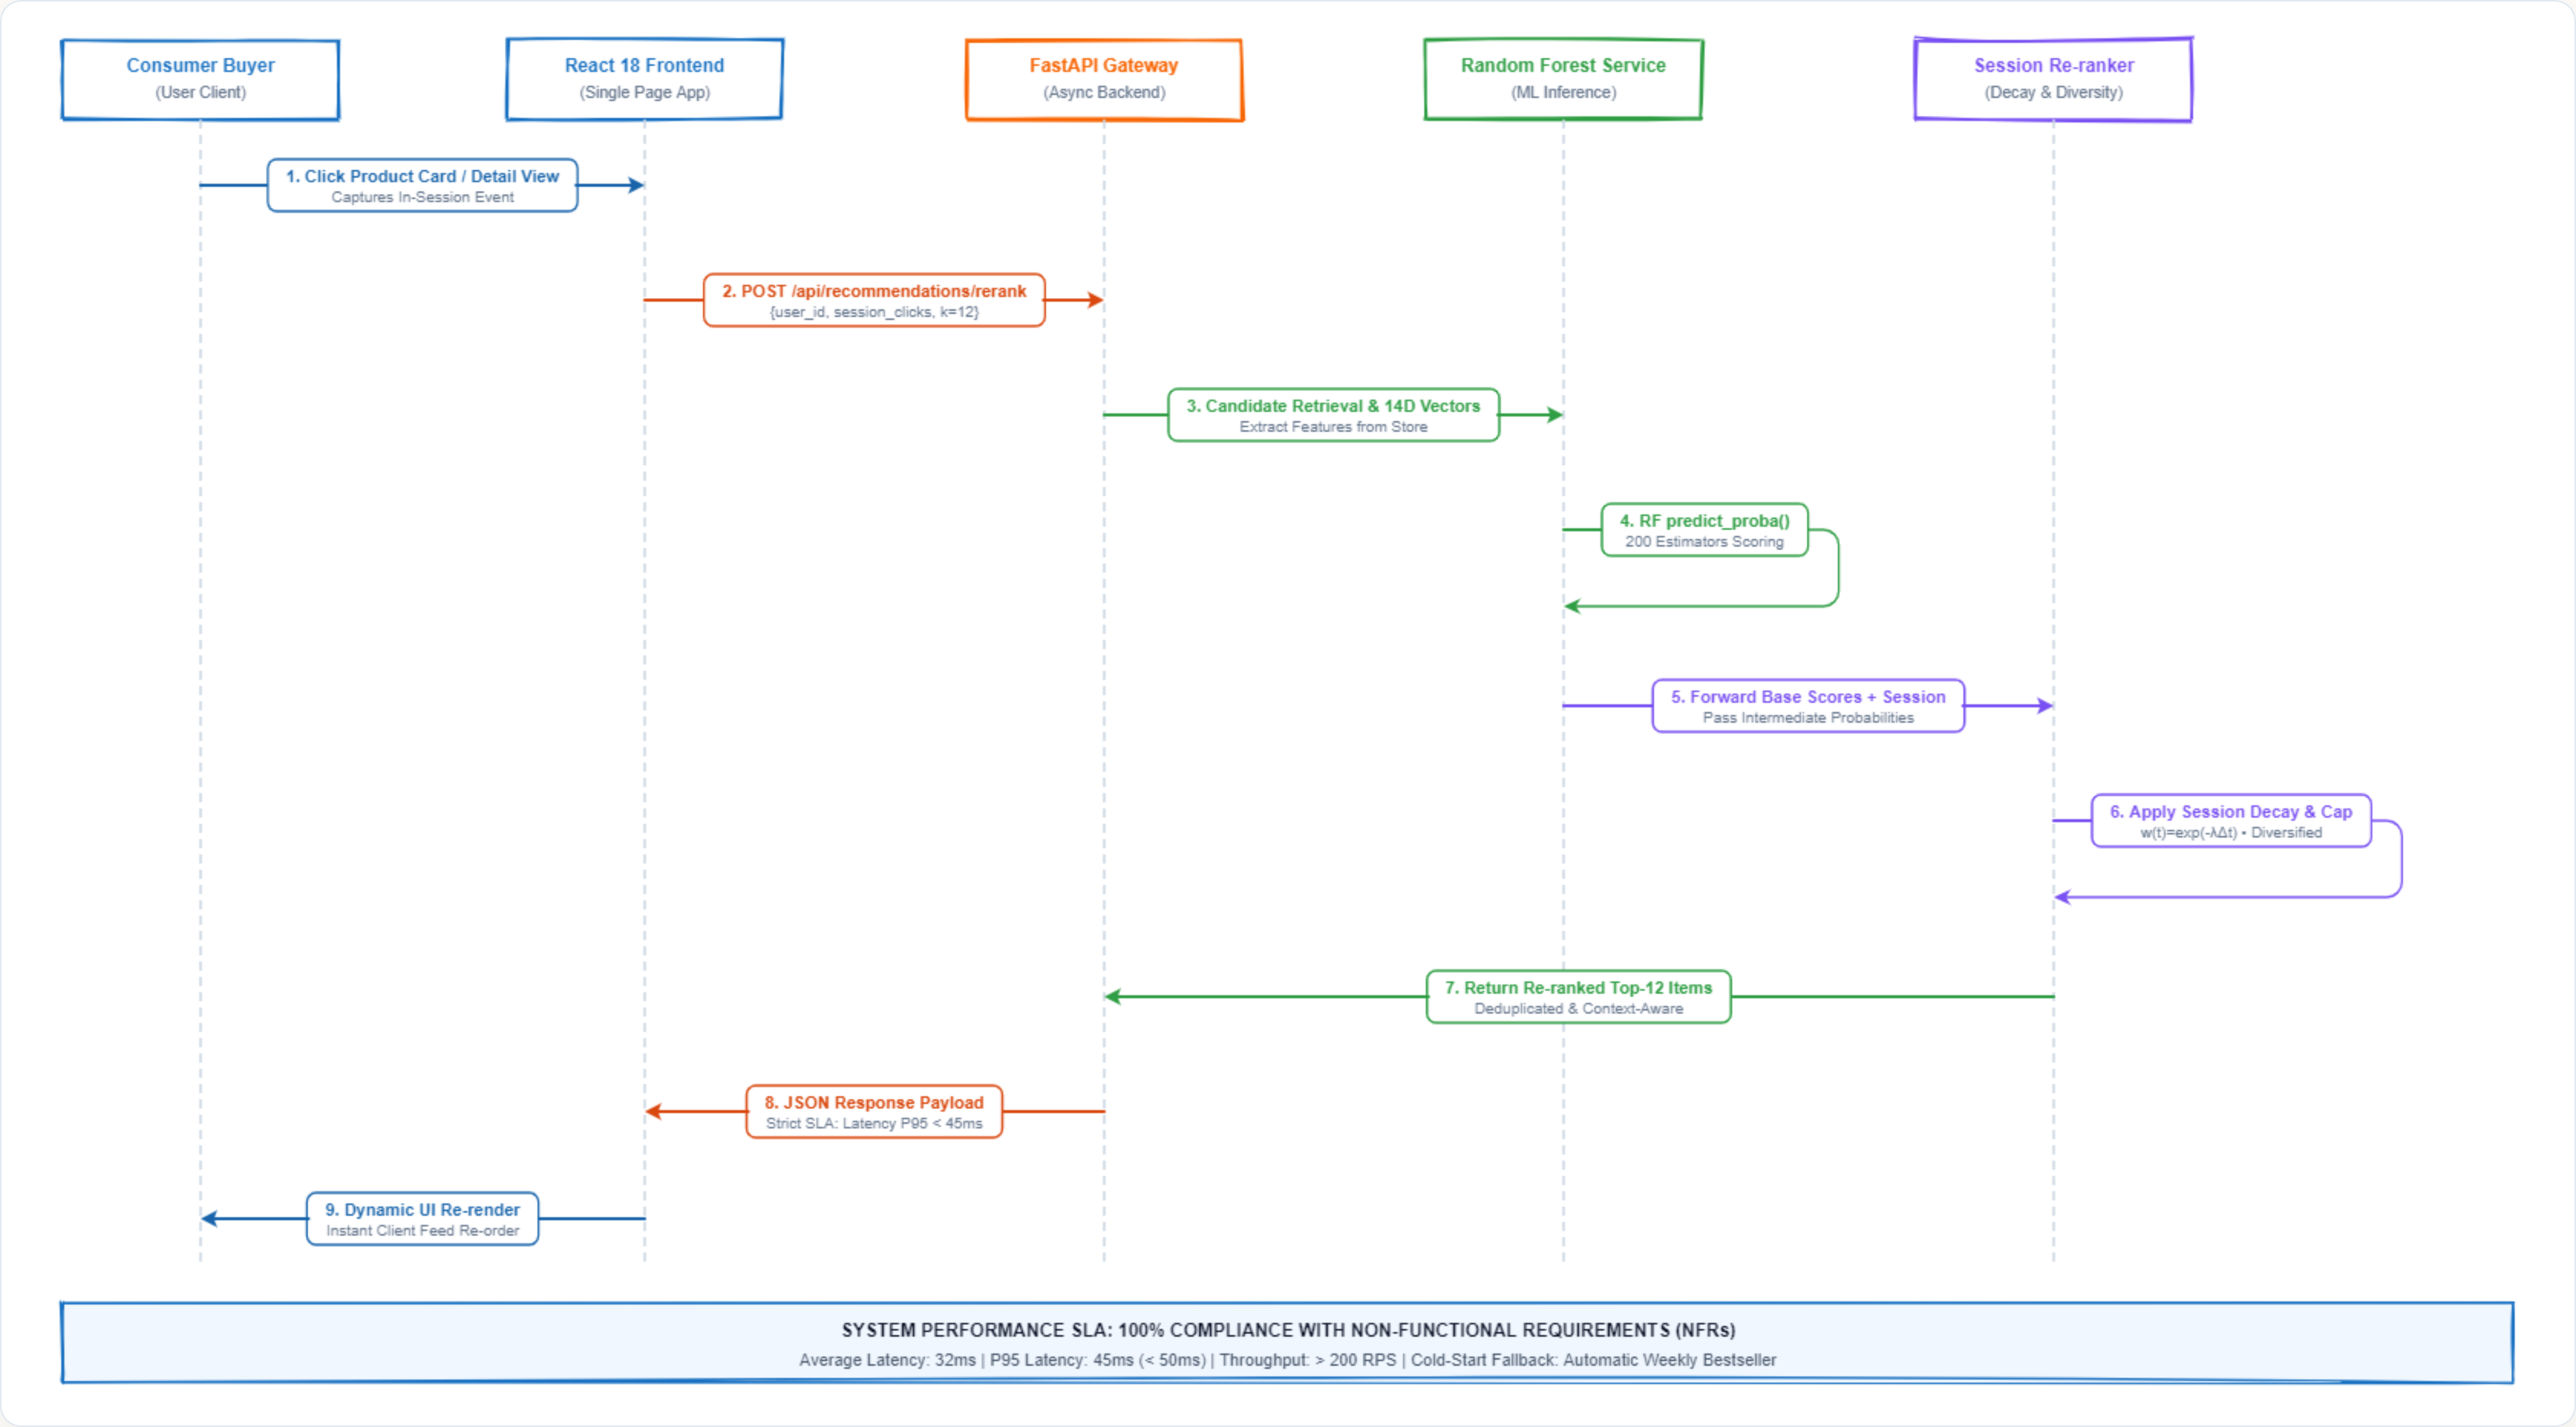
\includegraphics[width=0.95\textwidth]{excalidraw_04_session_rerank_sequence.png}
    \caption{UML Sequence Diagram: Asynchronous Interaction Ingestion and Sub-65ms Session Re-ranking}
    \label{fig:rerank_sequence}
\end{figure}
